\documentclass[UTF8,a4paper,11pt,fontset=fandol]{ctexart}
\usepackage{geometry}
\geometry{margin=2.2cm}
\usepackage{amsmath,amssymb,longtable,booktabs,array,hyperref,xcolor,enumitem,graphicx,float}
\hypersetup{colorlinks=true,linkcolor=blue,urlcolor=blue}
\setlist[itemize]{leftmargin=1.3em,itemsep=0.2em}
\definecolor{notegray}{RGB}{246,248,251}
\title{P15. D-HAL: Distributed Hierarchical Adversarial Learning for Multi-Agent Interaction in Autonomous Intersection Management\\中英双语博士精读笔记}
\author{Guanzhou Li; Jianping Wu; Yujing He}
\date{2023 · arXiv preprint}
\begin{document}
\maketitle

\noindent\textbf{Theme / 主题：} Distributed hierarchical learning for AIM\\
\textbf{Method family / 方法族：} Distributed hierarchical adversarial learning / 分布式层次化对抗学习\\
\textbf{PDF pages / 页数：} 17 \quad
\textbf{Relevance / 相关度：} 73/100\\
\textbf{Source / 来源：} \url{https://arxiv.org/abs/2303.02630}

\section{论文全景速览与核心贡献 / High-Level Overview \& Core Contributions}
\subsection{研究背景与痛点 / Background \& Pain Points}
这篇论文位于“Distributed hierarchical learning for AIM”方向。对你的 JSSP-based Intersection Management 课题，它回答的是高层调度、低层轨迹平滑、安全过滤或真实验证中的一个关键子问题：如何让车辆在路口少停、少冲突、少能耗，同时保持在线可执行。

The paper belongs to the theme of Distributed hierarchical learning for AIM. For a JSSP-based intersection-management thesis, it illuminates one of the key layers: scheduling, smoothing, safety filtering, or real-world validation.

\textbf{Pain point / 痛点：} Learning framework lacks explicit optimization/smoothing formulation and formal safety guarantees.

\subsection{核心科学问题 / Core Scientific Question}
如何用层次化长期/短期判别机制改进多智能体交叉口交互策略学习？

How can hierarchical long-term and short-term adversarial discrimination improve multi-agent interaction learning for AIM?

\subsection{科学贡献 / Scientific Contributions}
\begin{itemize}
\item 方法贡献 (method contribution)：Non-RL adversarial actor/discriminator framework evaluates immediate interaction and final trajectory quality for multi-agent AIM.
\item 安全/避碰贡献 (safety contribution)：Immediate and final discriminators score interaction safety and trajectory outcomes.
\item 平滑/停止避免贡献 (smoothing contribution)：Targets reduced travel time and smoother interaction outcomes compared with distributed learning baselines.
\item 创新力度评判 (reviewer judgement)：中等偏强：层次化对抗学习有新意，但安全和可解释性仍弱于约束优化方法。
\end{itemize}


\subsection{核心概念对照 / Core Concepts}
\begin{longtable}{p{0.24\linewidth}p{0.28\linewidth}p{0.40\linewidth}}
\toprule
中文概念 & English Concept & Role / 学术作用\\
\midrule
自动交叉口管理 & Autonomous Intersection Management & 把信号控制替换为车辆级调度与控制。 \\
轨迹平滑 & Trajectory Smoothing & 减少急加减速、停车和能耗峰值。 \\
安全约束 & Safety Constraints & 把碰撞风险写成距离、时间间隔或屏障函数。 \\
Distributed hierarchical adversarial learning & 分布式层次化对抗学习 & 该论文的核心方法族。 \\
\bottomrule
\end{longtable}

\section{教材式学习路径与关键截图 / Textbook-Style Study Path \& PDF Snapshots}
\subsection{学习路径 / Study Path}
\begin{itemize}
\item 第一遍先读首页截图、摘要与引言，确认研究问题和场景假设。
\item 第二遍沿着技术路线图复现模型变量、约束和求解器输入输出。
\item 第三遍逐节阅读 section deep reading，对照 PDF 截图检查公式、图表和实验。
\item 第四遍只站在审稿人视角重读实验，判断 baseline、公平性、消融和鲁棒性。
\item 最后把博士 checklist 写成自己的复现实验或论文拓展计划。
\end{itemize}


\subsection{博士阅读 Checklist / Doctoral Reading Checklist}
\begin{itemize}
\item 能否独立重写核心公式：层次对抗学习目标 / Hierarchical adversarial-learning objective，并解释每个符号的物理意义？
\item 能否画出输入-模型-算法-控制-验证的数据流图？
\item 能否指出至少两个强假设，并说明它们在真实交通中何时失效？
\item 能否复述实验基准是否公平，指标是否覆盖效率、安全、能耗和计算时间？
\item 能否提出一个与自己 JSSP/RL/smoother 课题直接相连的拓展实验？
\end{itemize}


\subsection{关键截图讲解 / PDF Snapshot Explanation}
Screenshots are selected anchors from the local PDFs for study and parallel reading. They do not replace the original paper.

\begin{figure}[H]
\centering

\includegraphics[width=0.92\linewidth]{../../assets/P15_li2023dhal/01_title_and_abstract_p1.jpg}
\caption{首页与摘要 / Title and abstract page (p.1, full\_page). 这张截图用于把笔记中的抽象概念拉回原论文页面，便于你平行阅读原文、公式、图表和实验设置。 与当前课题的连接：Useful for explaining why learned interaction policies must still be checked by a low-level feasibility/safety layer.}
\end{figure}

\begin{figure}[H]
\centering

\includegraphics[width=0.92\linewidth]{../../assets/P15_li2023dhal/02_modeling_or_problem_setup_p4.jpg}
\caption{建模或问题设定页 / Modeling or problem-setup page (p.4, full\_page). 这张截图用于把笔记中的抽象概念拉回原论文页面，便于你平行阅读原文、公式、图表和实验设置。 与当前课题的连接：Useful for explaining why learned interaction policies must still be checked by a low-level feasibility/safety layer.}
\end{figure}

\begin{figure}[H]
\centering

\includegraphics[width=0.92\linewidth]{../../assets/P15_li2023dhal/03_core_method_or_algorithm_p2.jpg}
\caption{核心方法或算法页 / Core method or algorithm page (p.2, full\_page). 这张截图用于把笔记中的抽象概念拉回原论文页面，便于你平行阅读原文、公式、图表和实验设置。 与当前课题的连接：Useful for explaining why learned interaction policies must still be checked by a low-level feasibility/safety layer.}
\end{figure}

\begin{figure}[H]
\centering

\includegraphics[width=0.92\linewidth]{../../assets/P15_li2023dhal/04_experiments_or_results_p9.jpg}
\caption{实验或结果页 / Experiments or results page (p.9, figure\_crop). 这张截图用于把笔记中的抽象概念拉回原论文页面，便于你平行阅读原文、公式、图表和实验设置。 与当前课题的连接：Useful for explaining why learned interaction policies must still be checked by a low-level feasibility/safety layer.}
\end{figure}

\begin{figure}[H]
\centering
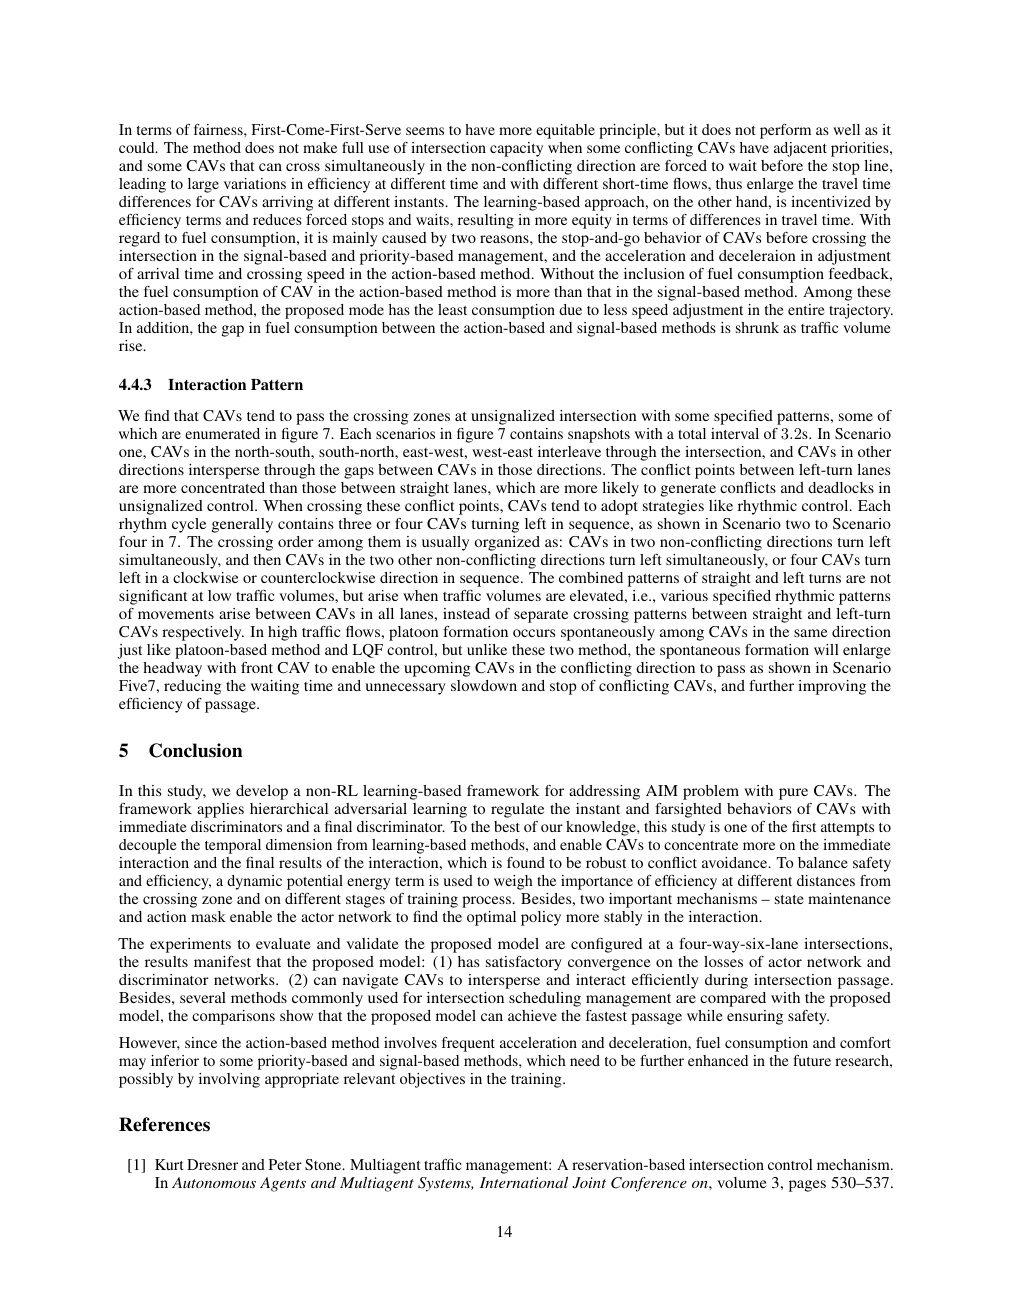
\includegraphics[width=0.92\linewidth]{../../assets/P15_li2023dhal/05_conclusion_or_limitations_p14.jpg}
\caption{结论或局限页 / Conclusion or limitations page (p.14, full\_page). 这张截图用于把笔记中的抽象概念拉回原论文页面，便于你平行阅读原文、公式、图表和实验设置。 与当前课题的连接：Useful for explaining why learned interaction policies must still be checked by a low-level feasibility/safety layer.}
\end{figure}


\section{章节精读与逐段导读 / Section-by-Section Deep Reading \& Walkthrough}
\subsection*{p.1 1 Introduction}
\textbf{章节目标 / Learning goal：} 建立研究动机：为什么传统信号控制、FCFS 或单车控制不足以处理该论文关注的交叉口协同问题。

Understand why the paper needs a new coordination method rather than a standard signal, FCFS, or single-vehicle controller.

\textbf{关键论点 / Key argument：} 这一部分通常把痛点落到 Distributed hierarchical learning for AIM：既要提高效率，又要保持安全与在线可执行。

\textbf{技术焦点 / Technical focus：} 精读时标出作者批判的 baseline、场景假设、交通参与者类型和隐含优化目标。

\textbf{审稿追问 / Reviewer question：} 作者指出的痛点是否真的需要新方法，还是可以由更强的优化器/更保守规则解决？

\subsection*{p.2 1. A hierarchical adversarial learning by long-term and short-term discrimination is adopted to realize the}
\textbf{章节目标 / Learning goal：} 承接前后章节，补充局部定义、案例或实现细节。

Recover implementation details needed for reproduction.

\textbf{关键论点 / Key argument：} 这类章节常常不是主贡献，但决定你能否真正复现方法。

\textbf{技术焦点 / Technical focus：} 检查它是否给出了参数、伪代码、场景划分或实现细节。

\textbf{审稿追问 / Reviewer question：} 跳过该节会不会导致公式或实验无法复现？

\subsection*{p.2 2. Potential energy method is applied to balance speed acquisition (efficiency) and conflict-avoidance (safety) in}
\textbf{章节目标 / Learning goal：} 解释算法如何把模型转化为可执行决策，并说明在线运行机制。

Trace how the paper turns the model into executable online decisions.

\textbf{关键论点 / Key argument：} D-HAL 通过长期和短期判别器引导策略学习，让智能体既模仿/区分整体交互轨迹，又修正局部短时动作。层次化目标试图改善多智能体交互中的稀疏奖励和非平稳性。

\textbf{技术焦点 / Technical focus：} 画出输入、核心求解器、输出和安全检查接口，明确哪些步骤是优化、哪些是规则、哪些是学习。

\textbf{审稿追问 / Reviewer question：} 若算法某一步失败，论文有没有 fallback、重规划或安全过滤机制？

\subsection*{p.2 2 Literature Review}
\textbf{章节目标 / Learning goal：} 建立方法谱系和相关工作边界，避免把本文贡献误读为完全从零开始。

Place the paper inside the broader method taxonomy.

\textbf{关键论点 / Key argument：} 该部分说明作者站在哪些已有工作之上，以及本文选择绕开或继承了哪些限制。

\textbf{技术焦点 / Technical focus：} 把相关工作按 scheduler、smoother、safety filter、evaluation 四类重排。

\textbf{审稿追问 / Reviewer question：} 作者是否公平比较了最接近的强 baseline？

\subsection*{p.4 3 Methodology}
\textbf{章节目标 / Learning goal：} 解释算法如何把模型转化为可执行决策，并说明在线运行机制。

Trace how the paper turns the model into executable online decisions.

\textbf{关键论点 / Key argument：} D-HAL 通过长期和短期判别器引导策略学习，让智能体既模仿/区分整体交互轨迹，又修正局部短时动作。层次化目标试图改善多智能体交互中的稀疏奖励和非平稳性。

\textbf{技术焦点 / Technical focus：} 画出输入、核心求解器、输出和安全检查接口，明确哪些步骤是优化、哪些是规则、哪些是学习。

\textbf{审稿追问 / Reviewer question：} 若算法某一步失败，论文有没有 fallback、重规划或安全过滤机制？

\subsection*{p.4 3.1 Problem Statement}
\textbf{章节目标 / Learning goal：} 把自然语言交通问题压缩为变量、状态、约束、目标函数或图结构。

Translate the traffic problem into variables, states, constraints, objectives, or graph relations.

\textbf{关键论点 / Key argument：} 本节是复现论文的核心入口，应与公式“层次对抗学习目标 / Hierarchical adversarial-learning objective”一起读。

\textbf{技术焦点 / Technical focus：} 逐项检查车辆状态、冲突关系、控制输入、时间/空间索引和安全阈值是否定义完整。

\textbf{审稿追问 / Reviewer question：} 这些建模假设在混合交通、通信延迟、感知误差和高密度车流下是否仍成立？

\subsection*{p.5 3.3 Reservation Mechanism}
\textbf{章节目标 / Learning goal：} 承接前后章节，补充局部定义、案例或实现细节。

Recover implementation details needed for reproduction.

\textbf{关键论点 / Key argument：} 这类章节常常不是主贡献，但决定你能否真正复现方法。

\textbf{技术焦点 / Technical focus：} 检查它是否给出了参数、伪代码、场景划分或实现细节。

\textbf{审稿追问 / Reviewer question：} 跳过该节会不会导致公式或实验无法复现？

\subsection*{p.6 3.4 Hierarchical Adversarial Learning}
\textbf{章节目标 / Learning goal：} 承接前后章节，补充局部定义、案例或实现细节。

Recover implementation details needed for reproduction.

\textbf{关键论点 / Key argument：} 这类章节常常不是主贡献，但决定你能否真正复现方法。

\textbf{技术焦点 / Technical focus：} 检查它是否给出了参数、伪代码、场景划分或实现细节。

\textbf{审稿追问 / Reviewer question：} 跳过该节会不会导致公式或实验无法复现？


\subsection{逐段式导读 / Paragraph-Level Walkthrough}
\paragraph{Opening motivation / 开篇动机段}先把作者的痛点翻译成一句博士问题：如何用层次化长期/短期判别机制改进多智能体交叉口交互策略学习？ 读这一段时不要急着接受动机，要追问传统 FCFS、信号灯或保守 MPC 为什么不足。

Turn the opening motivation into one doctoral-level question and test whether the paper truly needs a new method.

\paragraph{Assumption and setting / 假设与场景段}把车辆类型、通信条件、路口类型和动力学假设列成表。该文的关键边界包括：专家轨迹或高质量行为分布可用于判别学习。；长期/短期判别目标与真实交通安全效率一致。；仿真环境足以覆盖多智能体交互复杂性。

List vehicle type, communication, intersection setting, and dynamics assumptions before reading the equations.

\paragraph{Model and notation / 模型与符号段}围绕核心公式“层次对抗学习目标 / Hierarchical adversarial-learning objective”复写符号表，确认每个变量是决策变量、状态变量、参数还是约束阈值。

Rewrite the symbol table around the core formulation and classify variables as states, decisions, parameters, or constraints.

\paragraph{Algorithm mechanism / 算法机制段}把算法读成一条数据流：输入交通状态，执行 Non-RL adversarial actor/discriminator framework evaluates immediate interaction and final trajectory quality for multi-agent AIM.，输出可执行通行/控制决策，并检查安全接口。

Read the algorithm as a dataflow from traffic state to executable sequence/control decision, with explicit safety interfaces.

\paragraph{Experiment and evidence / 实验证据段}不要只看作者报告的提升，要检查基准、公平性和指标。本文验证描述为：Four-way six-lane intersection experiments against state-of-the-art methods.

Go beyond reported gains and inspect baselines, fairness, metrics, and computation time.

\paragraph{Reviewer synthesis / 审稿式总结段}最后把贡献拆成可发表与需补强两部分。对你课题最直接的用途是：Useful for explaining why learned interaction policies must still be checked by a low-level feasibility/safety layer.

Separate publishable contribution from missing evidence, then connect the result to your own thesis architecture.


\section{技术路线图与贡献量评估 / Technical Route \& Contribution Matrix}
\begin{longtable}{p{0.08\linewidth}p{0.24\linewidth}p{0.58\linewidth}}
\toprule
Step & Stage / 阶段 & Content / 内容\\
\midrule
1 & 输入 / Input & 车辆状态、路径/车道、交通需求、信号或协同信息。 \\
2 & 建模 / Modeling & 层次对抗学习目标 / Hierarchical adversarial-learning objective \\
3 & 核心求解 / Core solver & Non-RL adversarial actor/discriminator framework evaluates immediate interaction and final trajectory quality for multi-agent AIM. \\
4 & 安全接口 / Safety interface & Immediate and final discriminators score interaction safety and trajectory outcomes. \\
5 & 平滑与效率 / Smoothing and efficiency & Targets reduced travel time and smoother interaction outcomes compared with distributed learning baselines. \\
6 & 验证 / Validation & Four-way six-lane intersection experiments against state-of-the-art methods. \\
\bottomrule
\end{longtable}

\begin{longtable}{p{0.34\linewidth}p{0.14\linewidth}p{0.42\linewidth}}
\toprule
Dimension / 维度 & Score & Comment / 评语\\
\midrule
理论贡献 / Theoretical contribution & 3/5 & 层次对抗学习目标 / Hierarchical adversarial-learning objective \\
算法贡献 / Algorithmic contribution & 5/5 & Non-RL adversarial actor/discriminator framework evaluates immediate interaction and final trajectory quality for multi-agent AIM. \\
实验贡献 / Experimental contribution & 3/5 & Four-way six-lane intersection experiments against state-of-the-art methods. \\
工程贡献 / Engineering contribution & 3/5 & Immediate and final discriminators score interaction safety and trajectory outcomes. \\
博士课题价值 / PhD relevance & 4/5 & Useful for explaining why learned interaction policies must still be checked by a low-level feasibility/safety layer. \\
\bottomrule
\end{longtable}

\section{理论方法论深度解构 / Methodology \& Theoretical Framework}
\subsection{问题数学建模 / Mathematical Formulation}
\textbf{层次对抗学习目标 / Hierarchical adversarial-learning objective}
\[
\min_{\pi}\max_{D_L,D_S}\; \mathbb{E}_{\tau\sim\pi_E}[\log D(\tau)]+\mathbb{E}_{\tau\sim\pi}[\log(1-D(\tau))]-\lambda J_{RL}(\pi)
\]
\begin{longtable}{p{0.16\linewidth}p{0.25\linewidth}p{0.25\linewidth}p{0.25\linewidth}}
\toprule
Symbol / 符号 & 含义 & Meaning & Role / 建模作用\\
\midrule
pi & 多智能体策略 & multi-agent policy & 学习车辆交互行为 \\
D\_L & 长期判别器 & long-term discriminator & 评价轨迹级行为质量 \\
D\_S & 短期判别器 & short-term discriminator & 评价局部交互动作 \\
tau & 轨迹片段 & trajectory segment & 对抗学习样本 \\
J\_RL & 强化学习收益 & RL return & 保留任务奖励优化目标 \\
\bottomrule
\end{longtable}

\subsection{核心算法架构 / Core Algorithm Layout}
D-HAL 通过长期和短期判别器引导策略学习，让智能体既模仿/区分整体交互轨迹，又修正局部短时动作。层次化目标试图改善多智能体交互中的稀疏奖励和非平稳性。

D-HAL uses long-term and short-term discriminators to shape multi-agent policies, improving interaction learning under sparse rewards and non-stationarity.

\subsection{收敛性、稳定性或实时性 / Convergence, Stability, Real-Time Feasibility}
对抗训练可能提升样本效率，但也会带来训练不稳定；安全仍主要通过奖励或环境终止惩罚表达，缺少硬约束。

Adversarial training can improve sample efficiency but may be unstable; safety is still mostly reward-based unless paired with constraints.

\subsection{潜在假设与边界条件 / Assumptions \& Boundary Conditions}
\begin{itemize}
\item 专家轨迹或高质量行为分布可用于判别学习。
\item 长期/短期判别目标与真实交通安全效率一致。
\item 仿真环境足以覆盖多智能体交互复杂性。
\end{itemize}


\section{实验验证与结果评判 / Experimental Validation \& Result Evaluation}
\textbf{Baselines \& Environment / 基准与环境：} 普通 MARL、模仿学习、无层次判别器版本、无对抗损失版本。

\textbf{Validation / 验证：} Four-way six-lane intersection experiments against state-of-the-art methods.

\textbf{Metrics / 指标：} 碰撞率、平均延误、通行效率、成功率、奖励曲线和训练样本效率。

\textbf{Ablation / 消融：} 必须拆分长期判别器、短期判别器、对抗损失和 RL 任务损失；否则难以证明层次结构必要。

\textbf{Reviewer reading / 审稿式阅读提醒：} 阅读实验时不要只看平均值；应检查交通密度、车流方向、随机种子、失败案例和计算耗时。For doctoral reading, inspect density regimes, demand patterns, random seeds, failure cases, and computation time rather than only mean improvements.

\subsection{图表阅读线索 / Figure and Table Reading Cues}
PDF extraction detected approximately 8 figure references and 6 table references. Exact captions remain in the original PDF; the bilingual cues below tell you what to inspect first.

\begin{longtable}{p{0.24\linewidth}p{0.30\linewidth}p{0.36\linewidth}}
\toprule
图表名称 & Figure/Table Name & Reading focus / 阅读重点\\
\midrule
系统框架图 & system framework diagram & 先确认输入、决策层、控制层和安全约束之间的数据流。 \\
策略网络/训练流程图 & policy-network or training-pipeline diagram & 检查状态、动作、奖励、经验回放和安全惩罚是否闭环一致。 \\
实验指标对比图表 & experimental metric comparison plots/tables & 重点看平均值之外的密度变化、失败场景、计算时间和方差。 \\
\bottomrule
\end{longtable}

\section{审稿人视角：批判性思考与未来方向 / Critical Thinking \& Future Directions}
\subsection{论文局限性 / Limitations \& Weaknesses}
\begin{itemize}
\item 对抗训练难调参，复现实验成本高。
\item 策略可解释性弱，审稿人会追问安全证书。
\item 分布式学习结果可能依赖仿真器和奖励设置。
\end{itemize}


\subsection{博士课题拓展点 / Research Extensions for PhD}
\begin{itemize}
\item 用 JSSP 求解器生成专家排序轨迹，训练 imitation/adversarial scheduler。
\item 把判别器输出作为调度质量估计，而不是直接控制车辆。
\item 在对抗学习外加 CBF/MPC 安全约束，分离效率学习与安全保证。
\end{itemize}


\subsection{如何服务当前课题 / Use in This Project}
Useful for explaining why learned interaction policies must still be checked by a low-level feasibility/safety layer.

\section{交互式可视化与 PDF 排版蓝图 / Interactive Visualization \& PDF Layout Blueprint}
\textbf{动态参数 / Parameter：} 对抗损失权重 / Adversarial loss weight, range [0, 3] .

权重适中可提升交互拟合，过高会牺牲任务奖励稳定性。

Moderate weight improves interaction shaping; too much can destabilize RL.

\subsection{HTML 结构化布局建议 / HTML Structuring}
\begin{itemize}
\item 顶部固定 metadata bar：题名、作者、年份、主题、PDF 页数。
\item 左侧目录/section navigator，右侧为五大精读模块。
\item 公式卡片使用 <pre> 或 LaTeX block，紧跟符号表。
\item 审稿人批注用 reviewer-note block，博士拓展用 research-idea list。
\item 交互参数用 input[type=range] + canvas 曲线，打印 PDF 时隐藏交互控件但保留解释。
\end{itemize}


\section{来源锚点与逐节阅读路径 / Source Anchors \& Section-by-Section Reading Map}
\begin{longtable}{p{0.14\linewidth}p{0.76\linewidth}}
\toprule
Page & Extracted heading\\
\midrule
p.1 & 1 Introduction \\
p.2 & 2. Potential energy method is applied to balance speed acquisition (efficiency) and conflict-avoidance (safety) in \\
p.9 & 4 Experiments \\
\bottomrule
\end{longtable}

\paragraph{p.1 1 Introduction}定位问题背景、研究缺口和为什么现有保守/非协同方法不足。 / Frames the motivation, research gap, and limits of conservative or non-cooperative methods.

\paragraph{p.2 1. A hierarchical adversarial learning by long-term and short-term discrimination is adopted to realize the}作为局部论证段落阅读，关注它如何服务主问题。 / Read as a local argument and ask how it supports the main question.

\paragraph{p.2 2. Potential energy method is applied to balance speed acquisition (efficiency) and conflict-avoidance (safety) in}给出算法流程和求解机制，应重点追踪输入、输出和安全接口。 / Gives the algorithmic mechanism; track inputs, outputs, and safety interfaces.

\paragraph{p.2 2 Literature Review}作为局部论证段落阅读，关注它如何服务主问题。 / Read as a local argument and ask how it supports the main question.

\paragraph{p.4 3 Methodology}给出算法流程和求解机制，应重点追踪输入、输出和安全接口。 / Gives the algorithmic mechanism; track inputs, outputs, and safety interfaces.

\paragraph{p.4 3.1 Problem Statement}把交通交互转写为状态、约束、目标或图结构，是精读时最应复现的部分。 / Defines states, constraints, objectives, or graph structures; this is the section to reproduce carefully.

\paragraph{p.5 3.3 Reservation Mechanism}作为局部论证段落阅读，关注它如何服务主问题。 / Read as a local argument and ask how it supports the main question.

\paragraph{p.6 3.4 Hierarchical Adversarial Learning}作为局部论证段落阅读，关注它如何服务主问题。 / Read as a local argument and ask how it supports the main question.


\end{document}
